% Created 2022-08-28 dom 13:33
% Intended LaTeX compiler: pdflatex
\documentclass[t, aspectratio=169]{beamer}
\usepackage[utf8]{inputenc}
\usepackage[T1]{fontenc}
\usepackage{graphicx}
\usepackage{longtable}
\usepackage{wrapfig}
\usepackage{rotating}
\usepackage[normalem]{ulem}
\usepackage{amsmath}
\usepackage{amssymb}
\usepackage{capt-of}
\usepackage{hyperref}
\usepackage[newfloat]{minted}
\usepackage{tikz}
\usetikzlibrary{calc, tikzmark}
\usepackage{booktabs}
\usetheme{default}
\author{Luigi D. C. Soares}
\date{DCC/UFMG (30/08/2022)}
\title{Variáveis e Tipos}
\subtitle{Progamação e Desenvolvimento de Software I}
\title[Variáveis e Tipos]{Variáveis e Tipos}
\subtitle{Programação e Desenvolvimento de Software I}
\author[\tiny\{gleison.mendonca, luigi.domenico\}@dcc.ufmg.br]{%
Gleison S. D. Mendonça, Luigi D. C. Soares\texorpdfstring{\\}{}
\texttt{\{gleison.mendonca, luigi.domenico\}@dcc.ufmg.br}}
\institute[DCC/UFMG]{}
\date[30/08/2022]{}
%\usetheme{saori}
%\usemintedstyle{native}
\usetheme{ufmg}
\hypersetup{
 pdfauthor={Luigi D. C. Soares},
 pdftitle={Variáveis e Tipos},
 pdfkeywords={},
 pdfsubject={},
 pdfcreator={Emacs 28.1 (Org mode 9.6)}, 
 pdflang={English}}
\begin{document}

\maketitle

\begin{frame}[label={sec:org5d3b95a}]{Notação Decimal vs Binária}
\begin{itemize}
\item Decompondo um número representado na notação decimal
\end{itemize}

\begin{align*}
    {\color{highlight}19}{\color{blue!80}.625}
    =\;& \phantom{{\color{highlight}1} \times 10^{1} +
         {\color{highlight}9} \times 10^{0} +
         {\color{blue!80}6} \times 10^{-1} +
         {\color{blue!80}2} \times 10^{-2} +
         {\color{blue!80}5} \times 10^{-3}}
\end{align*}
\end{frame}

\begin{frame}[label={sec:orge093254}]{Notação Decimal vs Binária}
\begin{itemize}
\item Decompondo um número representado na notação decimal
\end{itemize}

\begin{align*}
    {\color{highlight}19}{\color{blue!80}.625}
    =\;& {\color{highlight}1} \times 10^{1} +
         {\color{highlight}9} \times 10^{0} +
         {\color{blue!80}6} \times 10^{-1} +
         {\color{blue!80}2} \times 10^{-2} +
         {\color{blue!80}5} \times 10^{-3}
\end{align*}
\end{frame}

\begin{frame}[label={sec:org51023e6}]{Notação Decimal vs Binária}
\begin{itemize}
\item Decompondo um número representado na notação decimal
\end{itemize}

\begin{align*}
    {\color{highlight}19}{\color{blue!80}.625}
    =\;& {\color{highlight}1} \times 10^{1} +
         {\color{highlight}9} \times 10^{0} +
         {\color{blue!80}6} \times 10^{-1} +
         {\color{blue!80}2} \times 10^{-2} +
         {\color{blue!80}5} \times 10^{-3} \\
    =\;& {\color{highlight}10} +
         {\color{highlight}9} +
         {\color{blue!80}0.6} +
         {\color{blue!80}0.02} +
         {\color{blue!80}0.005}
\end{align*}
\end{frame}

\begin{frame}[label={sec:orgda18026}]{Notação Decimal vs Binária}
\begin{itemize}
\item De binário para decimal
\end{itemize}

\begin{align*}
    {\color{highlight}10011}\color{blue!80}.101
    =\;& \phantom{{\color{highlight}1} \times 2^{4} +
         {\color{highlight}0} \times 2^{3} +
         {\color{highlight}0} \times 2^{2} +
         {\color{highlight}1} \times 2^{1} +
         {\color{highlight}1} \times 2^{0} +}
\end{align*}
\end{frame}

\begin{frame}[label={sec:orgaf0e6c5}]{Notação Decimal vs Binária}
\begin{itemize}
\item De binário para decimal
\end{itemize}

\begin{align*}
    {\color{highlight}10011}\color{blue!80}.101
    =\;& {\color{highlight}1} \times 2^{4} +
         {\color{highlight}0} \times 2^{3} +
         {\color{highlight}0} \times 2^{2} +
         {\color{highlight}1} \times 2^{1} +
         {\color{highlight}1} \times 2^{0} + \\
     \;& {\color{blue!80}1} \times 2^{-1} +
         {\color{blue!80}0} \times 2^{-2} +
         {\color{blue!80}1} \times 2^{-3}
\end{align*}
\end{frame}

\begin{frame}[label={sec:org94d2271}]{Notação Decimal vs Binária}
\begin{itemize}
\item De binário para decimal
\end{itemize}

\begin{align*}
    {\color{highlight}10011}\color{blue!80}.101
    =\;& {\color{highlight}1} \times 2^{4} +
         {\color{highlight}0} \times 2^{3} +
         {\color{highlight}0} \times 2^{2} +
         {\color{highlight}1} \times 2^{1} +
         {\color{highlight}1} \times 2^{0} + \\
     \;& {\color{blue!80}1} \times 2^{-1} +
         {\color{blue!80}0} \times 2^{-2} +
         {\color{blue!80}1} \times 2^{-3} \\
    =\;& {\color{highlight}16} +
         {\color{highlight}0} +
         {\color{highlight}0} +
         {\color{highlight}2} +
         {\color{highlight}1} +
         {\color{blue!80}0.5} +
         {\color{blue!80}0} +
         {\color{blue!80}0.125} \\
    =\;& {\color{highlight}19}{\color{blue!80}.625}
\end{align*}
\end{frame}

\begin{frame}[label={sec:org28ce497}]{Notação Decimal vs Binária}
\begin{itemize}
\item Caminho inverso: decimal para binário
\end{itemize}

\begin{alignat*}{2}
                        \quad 19& &&\; /\; 2 = \\
\end{alignat*}
\end{frame}

\begin{frame}[label={sec:orgf1d71bf}]{Notação Decimal vs Binária}
\begin{itemize}
\item Caminho inverso: decimal para binário
\end{itemize}

\begin{alignat*}{2}
                             19& &&\; /\; 2 = \\
    {\color{highlight}1}\quad 9& &&\; /\; 2 = \\
\end{alignat*}
\end{frame}

\begin{frame}[label={sec:orgf636943}]{Notação Decimal vs Binária}
\begin{itemize}
\item Caminho inverso: decimal para binário
\end{itemize}

\begin{alignat*}{2}
                             19& &&\; /\; 2 = \\
    {\color{highlight}1}\quad 9& &&\; /\; 2 = \\
    {\color{highlight}1}\quad 4& &&\; /\; 2 = \\
\end{alignat*}
\end{frame}

\begin{frame}[label={sec:orgdd0d476}]{Notação Decimal vs Binária}
\begin{itemize}
\item Caminho inverso: decimal para binário
\end{itemize}

\begin{alignat*}{2}
                             19& &&\; /\; 2 = \\
    {\color{highlight}1}\quad 9& &&\; /\; 2 = \\
    {\color{highlight}1}\quad 4& &&\; /\; 2 = \\
    {\color{highlight}0}\quad 2& &&\; /\; 2 = \\
\end{alignat*}
\end{frame}

\begin{frame}[label={sec:orgd0902e9}]{Notação Decimal vs Binária}
\begin{itemize}
\item Caminho inverso: decimal para binário
\end{itemize}

\begin{alignat*}{2}
                             19& &&\; /\; 2 = \\
    {\color{highlight}1}\quad 9& &&\; /\; 2 = \\
    {\color{highlight}1}\quad 4& &&\; /\; 2 = \\
    {\color{highlight}0}\quad 2& &&\; /\; 2 = \\
    {\color{highlight}0}\quad 1& &&\; /\; 2 = \\
\end{alignat*}
\end{frame}

\begin{frame}[label={sec:orgdd7d604}]{Notação Decimal vs Binária}
\begin{itemize}
\item Caminho inverso: decimal para binário
\end{itemize}

\begin{alignat*}{2}
                             19& &&\; /\; 2 = \\
    {\color{highlight}1}\quad 9& &&\; /\; 2 = \\
    {\color{highlight}1}\quad 4& &&\; /\; 2 = \\
    {\color{highlight}0}\quad 2& &&\; /\; 2 = \\
    {\color{highlight}0}\quad 1& &&\; /\; 2 = \\
    {\color{highlight}1}\quad 0 \\
\end{alignat*}
\end{frame}

\begin{frame}[label={sec:orgaa0c2b8}]{Notação Decimal vs Binária}
\begin{itemize}
\item Caminho inverso: decimal para binário
\end{itemize}

\begin{alignat*}{2}
                             19& &&\; /\; 2 = \\
    \tikzmark{end-i}{\color{highlight}1}\quad 9& &&\; /\; 2 = \\
    {\color{highlight}1}\quad 4& &&\; /\; 2 = \\
    {\color{highlight}0}\quad 2& &&\; /\; 2 = \\
    {\color{highlight}0}\quad 1& &&\; /\; 2 = \\
    \tikzmark{begin-i}{\color{highlight}1}\quad 0 \\
\end{alignat*}

\begin{tikzpicture}[overlay, remember picture]
    \draw[highlight, thick, ->] ($(pic cs:begin-i) + (-0.25, 0)$) -- ($(pic cs:end-i) + (-0.25, +0.25)$);
\end{tikzpicture}
\end{frame}

\begin{frame}[label={sec:orgb62b415}]{Notação Decimal vs Binária}
\begin{itemize}
\item Caminho inverso: decimal para binário
\end{itemize}

\begin{alignat*}{2}
        \phantom{1}&\phantom{+ \quad}0.625&& \; \times\; 2 = \\
\end{alignat*}
\end{frame}

\begin{frame}[label={sec:org1991899}]{Notação Decimal vs Binária}
\begin{itemize}
\item Caminho inverso: decimal para binário
\end{itemize}

\begin{alignat*}{2}
                             &\phantom{+ \quad}0.625&& \; \times\; 2 = \\
    {\color{blue!80}1} &+ \quad 0.25&& \; \times\; 2 = \\
\end{alignat*}
\end{frame}

\begin{frame}[label={sec:orgb5f93fd}]{Notação Decimal vs Binária}
\begin{itemize}
\item Caminho inverso: decimal para binário
\end{itemize}

\begin{alignat*}{2}
                             &\phantom{+ \quad}0.625&& \; \times\; 2 = \\
    {\color{blue!80}1} &+ \quad 0.25&& \; \times\; 2 = \\
    {\color{blue!80}0} &+ \quad 0.5&& \; \times\; 2 = \\
\end{alignat*}
\end{frame}

\begin{frame}[label={sec:orgfa5cbc3}]{Notação Decimal vs Binária}
\begin{itemize}
\item Caminho inverso: decimal para binário
\end{itemize}

\begin{alignat*}{2}
                             &\phantom{+ \quad}0.625&& \; \times\; 2 = \\
    {\color{blue!80}1} &+ \quad 0.25&& \; \times\; 2 = \\
    {\color{blue!80}0} &+ \quad 0.5&& \; \times\; 2 = \\
    {\color{blue!80}1} & +\quad 0\\
\end{alignat*}
\end{frame}

\begin{frame}[label={sec:org8f1cd67}]{Notação Decimal vs Binária}
\begin{itemize}
\item Caminho inverso: decimal para binário
\end{itemize}

\begin{alignat*}{2}
                             &\phantom{+ \quad}0.625&& \; \times\; 2 = \\
    \tikzmark{begin-f}{\color{blue!80}1} &+ \quad 0.25&& \; \times\; 2 = \\
    {\color{blue!80}0} &+ \quad 0.5&& \; \times\; 2 = \\
    \tikzmark{end-f}{\color{blue!80}1} & +\quad 0\\
\end{alignat*}

\begin{tikzpicture}[overlay, remember picture]
    \draw[blue!80, thick, ->] ($(pic cs:begin-f) + (-0.25, +0.25)$) -- ($(pic cs:end-f) + (-0.25, 0)$);
\end{tikzpicture}
\end{frame}

\begin{frame}[label={sec:org304565f}]{Notação Decimal vs Binária}
\begin{itemize}
\item \(0.6 =\; ?\)
\item Quantos bits precisamos depois do ``.''?
\end{itemize}
\end{frame}

\begin{frame}[label={sec:orgb744fd1}]{Notação Decimal vs Binária}
\begin{itemize}
\item \(0.6 =\; 0.10011001\ldots\)
\item Quantos bits precisamos depois do ``.''? \alert{Infinitos}
\end{itemize}

\begin{alignat*}{2}
                             &\phantom{+ \quad}\;\, 0.6&& \; \times\; 2 = \\
    {\color{blue!80}1} &+ \quad 0.2&& \; \times\; 2 = \\
    {\color{blue!80}0} &+ \quad 0.4&& \; \times\; 2 = \\
    {\color{blue!80}0} &+ \quad 0.8&& \; \times\; 2 = \\
    {\color{blue!80}1} &+ \quad 0.6&& \; \times\; 2 = \ldots\\
\end{alignat*}
\end{frame}

\begin{frame}[label={sec:org9b7d48d}]{Representando números inteiros}
\begin{itemize}
\item Forma mais simples: \alert{sinal-magnitude}
\begin{itemize}
\item O {\bfseries\color{highlight}bit mais significativo} corresponde ao sinal
\item Os demais correspondem ao valor absoluto do número
\end{itemize}
\end{itemize}
\end{frame}

\begin{frame}[label={sec:orgca2a64c}]{Representando números inteiros}
\begin{itemize}
\item Forma mais simples: \alert{sinal-magnitude}
\begin{itemize}
\item O {\bfseries\color{highlight}bit mais significativo} corresponde ao sinal
\item Os demais correspondem ao valor absoluto do número
\end{itemize}

\item Exemplo: considere uma representação usando cinco dígitos binários (\alert{bits})
\end{itemize}

\begin{columns}
\begin{column}{0.5\columnwidth}
\begin{center}
\begin{tabular}{*{2}{c}}
\toprule
\alert{Decimal} & \alert{Binário}\\
\midrule
\(+5\) & {\bfseries\color{highlight}0} 0101\\
\(-3\) & {\bfseries\color{highlight}1} 0011\\
\bottomrule
\end{tabular}
\end{center}
\end{column}

\begin{column}{0.5\columnwidth}
\begin{center}
\begin{tabular}{ll}
 & 00101 (+5)\\
+ & 10011 (-3)\\
\hline
 & 11000 (-8 ???)\\
\end{tabular}
\end{center}
\end{column}
\end{columns}
\end{frame}

\begin{frame}[label={sec:orgfda2b7c}]{Representando números inteiros}
\begin{itemize}
\item Forma mais simples: \alert{sinal-magnitude}
\begin{itemize}
\item O {\bfseries\color{highlight}bit mais significativo} corresponde ao sinal
\item Os demais correspondem ao valor absoluto do número
\end{itemize}

\item \alert{Desvantagens}:
\begin{itemize}
\item A representação dificulta os cálculos
\item Duas notações para o zero (\(+0\) e \(-0\))
\end{itemize}
\end{itemize}
\end{frame}

\begin{frame}[label={sec:orgf226c8f}]{Representando números inteiros}
\begin{itemize}
\item Forma mais utilizada: \alert{complemento de 2}
\begin{itemize}
\item Números positivos: idêntica à forma sinal-magnitude
\end{itemize}
\end{itemize}
\end{frame}

\begin{frame}[label={sec:orgf7d43a9}]{Representando números inteiros}
\begin{itemize}
\item Forma mais utilizada: \alert{complemento de 2}
\begin{itemize}
\item Números positivos: idêntica à forma sinal-magnitude
\item Números negativos: a representação se dá em dois passos
\begin{enumerate}
\item Inverter os bits (0 vira 1, 1 vira 0) da representação do número positvo
\item Somar 1 ao resultado
\end{enumerate}
\end{itemize}
\end{itemize}
\end{frame}

\begin{frame}[label={sec:orgcd5bf8e}]{Representando números inteiros}
\begin{itemize}
\item Forma mais utilizada: \alert{complemento de 2}
\begin{itemize}
\item Números positivos: idêntica à forma sinal-magnitude
\item Números negativos: a representação se dá em dois passos
\begin{enumerate}
\item Inverter os bits (0 vira 1, 1 vira 0) da representação do número positvo
\item Somar 1 ao resultado
\end{enumerate}
\end{itemize}
\end{itemize}

\begin{columns}
\begin{column}{0.5\columnwidth}
\begin{center}
\begin{tabular}{*{2}{c}}
\toprule
\alert{Decimal} & \alert{Binário}\\
\midrule
\(+6\) & {\bfseries\color{highlight}0} 0110\\
\(-6\) & {\bfseries\color{highlight}1} 1010\\
\(+5\) & {\bfseries\color{highlight}0} 0101\\
\(-3\) & {\bfseries\color{highlight}1} 1101\\
\bottomrule
\end{tabular}
\end{center}
\end{column}

\begin{column}{0.5\columnwidth}
\begin{center}
\begin{tabular}{ll}
 & 00101 (+5)\\
+ & 11101 (-3)\\
\hline
 & 00010  (+2)\\
\end{tabular}
\end{center}
\end{column}
\end{columns}
\end{frame}

\begin{frame}[label={sec:orgc307681}]{Representando números reais}
\begin{itemize}
\item Representação com ponto fixo: \(12,34\)
\item Representação com \alert{ponto (vírgula) flutuante}: \(0,1234 \times 10^{2}\)
\item A representação com ponto flutuante segue padrões internacionais
(IEEE-754 e IEC-559)
\end{itemize}
\end{frame}

\begin{frame}[label={sec:orgb8b7875}]{Representando dados não-numéricos}
TODO
\end{frame}

\begin{frame}[label={sec:orgaa63b5d}]{Escrevendo um programa em C}
\begin{itemize}
\item Inclusão dos cabeçalhos das bibliotecas que vamos utilizar
\end{itemize}
\end{frame}

\begin{frame}[label={sec:org2a0527b}]{Escrevendo um programa em C}
\begin{itemize}
\item Inclusão dos cabeçalhos das bibliotecas que vamos utilizar
\item Função principal (\alert{main}): ponto de entrada do programa
\end{itemize}
\end{frame}

\begin{frame}[label={sec:orgd398b8e}]{Escrevendo um programa em C}
\begin{itemize}
\item Inclusão dos cabeçalhos das bibliotecas que vamos utilizar
\item Função principal (\alert{main}): ponto de entrada do programa
\item A linguagem C é \alert{case sensitive}
\begin{itemize}
\item \alert{Main} ou \alert{MAIN}, por exemplo, provocam erros de sintaxe
\end{itemize}
\end{itemize}
\end{frame}

\begin{frame}[label={sec:org3478f31}]{Escrevendo um programa em C}
\begin{itemize}
\item Inclusão dos cabeçalhos das bibliotecas que vamos utilizar
\item Função principal (\alert{main}): ponto de entrada do programa
\item A linguagem C é \alert{case sensitive}
\begin{itemize}
\item \alert{Main} ou \alert{MAIN}, por exemplo, provocam erros de sintaxe
\end{itemize}
\item Escrever um programa em C corresponde a escrever o \alert{corpo} da função principal
\end{itemize}
\end{frame}

\begin{frame}[label={sec:org6c02b18}]{Escrevendo um programa em C}
\begin{itemize}
\item Inclusão dos cabeçalhos das bibliotecas que vamos utilizar
\item Função principal (\alert{main}): ponto de entrada do programa
\item A linguagem C é \alert{case sensitive}
\begin{itemize}
\item \alert{Main} ou \alert{MAIN}, por exemplo, provocam erros de sintaxe
\end{itemize}
\item Escrever um programa em C corresponde a escrever o \alert{corpo} da função principal
\item O \alert{corpo} de uma função sempre começa com abre-chaves \alert{\{} e termina com fecha-chaves \alert{\}}
\end{itemize}
\end{frame}

\begin{frame}[label={sec:orgb70583e}]{Escrevendo um programa em C}
\begin{itemize}
\item Inclusão dos cabeçalhos das bibliotecas que vamos utilizar
\item Função principal (\alert{main}): ponto de entrada do programa
\item A linguagem C é \alert{case sensitive}
\begin{itemize}
\item \alert{Main} ou \alert{MAIN}, por exemplo, provocam erros de sintaxe
\end{itemize}
\item Escrever um programa em C corresponde a escrever o \alert{corpo} da função principal
\item O \alert{corpo} de uma função sempre começa com abre-chaves \alert{\{} e termina com fecha-chaves \alert{\}}
\item Comandos devem terminar com ponto e vírgula \alert{;}
\end{itemize}
\end{frame}

\begin{frame}[label={sec:orgf018a2f},fragile]{Escrevendo um programa em C}
 \vspace{-0.5cm}
\begin{minted}[,frame=lines,framesep=2mm,linenos]{c}
#include <stdio.h> // Cabeçalho da biblioteca de entrada/saída
// Função main: ponto de entrada do programa ("//" indica um comentário)
int main(int argc, char *argv[]) {
    /*
      Corpo da função principal
      (comentário em múltiplas linhas)
     */
    return 0;
}
\end{minted}
\end{frame}

\begin{frame}[label={sec:org7b86131},fragile]{Variáveis}
 \vspace{-0.5cm}
\begin{minted}[,frame=lines,framesep=2mm,linenos]{c}
#include <stdio.h>
int main(int argc, char *argv[]) {
    int a = 7;
    int b = 3;
    int q = 0; // Inicializando quociente
    while (b <= a) {
        q = q + 1; // Somar 1 ao valor de q
        a = a - b; // Subtrair B do valor de A
    }
    // ...
    return 0;
}
\end{minted}
\end{frame}

\begin{frame}[label={sec:org935438f}]{Variáveis}
\begin{itemize}
\item Os dados de um programa precisam ser armazenados na \alert{memória} do computador
\end{itemize}
\end{frame}

\begin{frame}[label={sec:org1e85bb2}]{Variáveis}
\begin{itemize}
\item Os dados de um programa precisam ser armazenados na \alert{memória} do computador
\item Cada posição de memória possui um \alert{endereço}
\end{itemize}
\end{frame}

\begin{frame}[label={sec:orgf805ce5}]{Variáveis}
\begin{itemize}
\item Os dados de um programa precisam ser armazenados na \alert{memória} do computador
\item Cada posição de memória possui um \alert{endereço}
\item Uma variável é um \alert{nome simbólico} (ou etiqueta) de uma posição de memória
\end{itemize}
\end{frame}

\begin{frame}[label={sec:org0e1a331}]{Variáveis}
\begin{itemize}
\item Os dados de um programa precisam ser armazenados na \alert{memória} do computador
\item Cada posição de memória possui um \alert{endereço}
\item Uma variável é um \alert{nome simbólico} (ou etiqueta) de uma posição de memória
\end{itemize}
\vfill{}\vspace{0.575cm}
\begin{center}
\begin{tabular}{*{11}{c}}
\toprule
\alert{Variável} & \alert{Endereço} & \alert{\ldots{}} & \alert{b\textsubscript{24}} & \alert{b\textsubscript{25}} & \alert{b\textsubscript{26}} & \alert{b\textsubscript{27}} & \alert{b\textsubscript{28}} & \alert{b\textsubscript{29}} & \alert{b\textsubscript{30}} & \alert{b\textsubscript{31}}\\
\midrule
a & e\textsubscript{0} & 0 & 0 & 0 & 0 & 0 & 0 & 1 & 1 & 1\\
b & e\textsubscript{1} & 0 & 0 & 0 & 0 & 0 & 0 & 0 & 1 & 1\\
q & e\textsubscript{2} & 0 & 0 & 0 & 0 & 0 & 0 & 0 & 0 & 0\\
\bottomrule
\end{tabular}
\end{center}
\end{frame}

\begin{frame}[label={sec:orgc2fcf93}]{Variáveis}
\begin{itemize}
\item Os dados de um programa precisam ser armazenados na \alert{memória} do computador
\item Cada posição de memória possui um \alert{endereço}
\item Uma variável é um \alert{nome simbólico} (ou etiqueta) de uma posição de memória
\item Seu \alert{conteúdo pode variar} durante a execução do programa
\end{itemize}
\vfill{}
\begin{center}
\begin{tabular}{*{11}{c}}
\toprule
\alert{Variável} & \alert{Endereço} & \alert{\ldots{}} & \alert{b\textsubscript{24}} & \alert{b\textsubscript{25}} & \alert{b\textsubscript{26}} & \alert{b\textsubscript{27}} & \alert{b\textsubscript{28}} & \alert{b\textsubscript{29}} & \alert{b\textsubscript{30}} & \alert{b\textsubscript{31}}\\
\midrule
a & e\textsubscript{0} & 0 & 0 & 0 & 0 & 0 & 0 & 1 & \alert{0} & \alert{0}\\
b & e\textsubscript{1} & 0 & 0 & 0 & 0 & 0 & 0 & 0 & 1 & 1\\
q & e\textsubscript{2} & 0 & 0 & 0 & 0 & 0 & 0 & 0 & 0 & \alert{1}\\
\bottomrule
\end{tabular}
\end{center}
\end{frame}

\begin{frame}[label={sec:orgec5d36d}]{Variáveis}
\begin{itemize}
\item Deve ser definida antes de ser utilizada:
\end{itemize}
\end{frame}

\begin{frame}[label={sec:org31c48f8},fragile]{Variáveis}
 \begin{itemize}
\item Deve ser definida antes de ser utilizada:
\end{itemize}
\begin{minted}[,frame=lines,framesep=2mm,linenos]{c}
#include <stdio.h>
int main(int argc, char *argv[]) {
    // Error: 'X' undeclared (first use in this function)
    printf("X: %d\n", X);
    return 0;
}
\end{minted}
\end{frame}

\begin{frame}[label={sec:org6efb61d}]{Variáveis}
\begin{itemize}
\item Deve ser definida antes de ser utilizada: \alert{\color{highlight}tipo\_variável \color{blue!80}lista\_de\_variáveis}
\end{itemize}
\end{frame}

\begin{frame}[label={sec:orga125290},fragile]{Variáveis}
 \begin{itemize}
\item Deve ser definida antes de ser utilizada: \alert{\color{highlight}tipo\_variável \color{blue!80}lista\_de\_variáveis}
\end{itemize}
\begin{minted}[,frame=lines,framesep=2mm,linenos]{c}
#include <stdio.h>
int main(int argc, char *argv[]) {
    int x, y;
    x = 10;
    y = 20;
    printf("X: %d\n", x);
    printf("Y: %d\n", y);
    return 0;
}
\end{minted}
\end{frame}

\begin{frame}[label={sec:org3c29519}]{Variáveis}
\begin{itemize}
\item Deve ser definida antes de ser utilizada: \alert{\color{highlight}tipo\_variável \color{blue!80}lista\_de\_variáveis}
\item \color{black}Nome:
\begin{itemize}
\item \emph{Case sensitive} (letras maiúsculas e minúsculas são consideradas diferentes)
\end{itemize}
\end{itemize}
\end{frame}

\begin{frame}[label={sec:org7dbe2d6},fragile]{Variáveis}
 \begin{itemize}
\item Deve ser definida antes de ser utilizada: \alert{\color{highlight}tipo\_variável \color{blue!80}lista\_de\_variáveis}
\item \color{black}Nome:
\begin{itemize}
\item \emph{Case sensitive} (letras maiúsculas e minúsculas são consideradas diferentes)
\end{itemize}
\end{itemize}

\begin{minted}[,frame=lines,framesep=2mm,linenos]{c}
#include <stdio.h>
int main(int argc, char *argv[]) {
    int x = 10;
    /* Error: 'X' undeclared (first use in this function)
       Note que 'X' é diferente de 'x' */
    printf("X: %d\n", X);
    return 0;
}
\end{minted}
\end{frame}

\begin{frame}[label={sec:orgf6ef75f}]{Variáveis}
\begin{itemize}
\item Deve ser definida antes de ser utilizada: \alert{\color{highlight}tipo\_variável \color{blue!80}lista\_de\_variáveis}
\item \color{black}Nome:
\begin{itemize}
\item \emph{Case sensitive} (letras maiúsculas e minúsculas são consideradas diferentes)
\item Pode ter um ou mais caracteres
\item Deve iniciar com letras ou underscore (\_)
\end{itemize}
\end{itemize}
\end{frame}

\begin{frame}[label={sec:org4507db5},fragile]{Variáveis}
 \begin{itemize}
\item Deve ser definida antes de ser utilizada: \alert{\color{highlight}tipo\_variável \color{blue!80}lista\_de\_variáveis}
\item \color{black}Nome:
\begin{itemize}
\item \emph{Case sensitive} (letras maiúsculas e minúsculas são consideradas diferentes)
\item Pode ter um ou mais caracteres
\item Deve iniciar com letras ou underscore (\_)
\end{itemize}
\end{itemize}

\begin{minted}[,frame=lines,framesep=2mm,linenos]{c}
#include <stdio.h>
int main(int argc, char *argv[]) {
    // Error: expected identifier or ‘(’ before numeric constant
    int 1;
    return 0;
}
\end{minted}
\end{frame}

\begin{frame}[label={sec:orge559ae9}]{Variáveis}
\begin{itemize}
\item Deve ser definida antes de ser utilizada: \alert{\color{highlight}tipo\_variável \color{blue!80}lista\_de\_variáveis}
\item \color{black}Nome:
\begin{itemize}
\item \emph{Case sensitive} (letras maiúsculas e minúsculas são consideradas diferentes)
\item Pode ter um ou mais caracteres
\item Deve iniciar com letras ou underscore (\_)
\item Caracteres devem ser letras, números ou underscores
\end{itemize}
\end{itemize}
\end{frame}

\begin{frame}[label={sec:org5f7b851},fragile]{Variáveis}
 \begin{itemize}
\item Deve ser definida antes de ser utilizada: \alert{\color{highlight}tipo\_variável \color{blue!80}lista\_de\_variáveis}
\item \color{black}Nome:
\begin{itemize}
\item \emph{Case sensitive} (letras maiúsculas e minúsculas são consideradas diferentes)
\item Pode ter um ou mais caracteres
\item Deve iniciar com letras ou underscore (\_)
\item Caracteres devem ser letras, números ou underscores
\end{itemize}
\end{itemize}

\begin{minted}[,frame=lines,framesep=2mm,linenos]{c}
#include <stdio.h>
int main(int argc, char *argv[]) {
    // Error: expected ‘=’, ‘,’, ‘;’, ‘asm’ or
    // ‘__attribute__’ before numeric constant
    int teste.123;
    return 0;
}
\end{minted}
\end{frame}

\begin{frame}[label={sec:org3450d67}]{Variáveis}
\begin{itemize}
\item Deve ser definida antes de ser utilizada: \alert{\color{highlight}tipo\_variável \color{blue!80}lista\_de\_variáveis}
\item \color{black}Nome:
\begin{itemize}
\item \emph{Case sensitive} (letras maiúsculas e minúsculas são consideradas diferentes)
\item Pode ter um ou mais caracteres
\item Deve iniciar com letras ou underscore (\_)
\item Caracteres devem ser letras, números ou underscores
\item Palavras-chave não podem ser usadas como nomes
\end{itemize}
\end{itemize}
\end{frame}

\begin{frame}[label={sec:org07d7558},fragile]{Variáveis}
 \begin{itemize}
\item Deve ser definida antes de ser utilizada: \alert{\color{highlight}tipo\_variável \color{blue!80}lista\_de\_variáveis}
\item \color{black}Nome:
\begin{itemize}
\item \emph{Case sensitive} (letras maiúsculas e minúsculas são consideradas diferentes)
\item Pode ter um ou mais caracteres
\item Deve iniciar com letras ou underscore (\_)
\item Caracteres devem ser letras, números ou underscores
\item Palavras-chave não podem ser usadas como nomes
\end{itemize}
\end{itemize}

\begin{minted}[,frame=lines,framesep=2mm,linenos]{c}
#include <stdio.h>
int main(int argc, char *argv[]) {
    // Error: expected identifier or ‘(’ before ‘while’
    int while;
    return 0;
}
\end{minted}
\end{frame}

\begin{frame}[label={sec:orgcbd2408}]{Variáveis}
\begin{itemize}
\item Lista de palavras-chave: \alert{auto break case char const continue default do double}
\alert{else enum extern float for goto if int long register return short signed}
\alert{sizeof static struct switch typeof union unsigned void volatile while}
\end{itemize}
\end{frame}

\begin{frame}[label={sec:org717c00d}]{Variáveis}
\begin{itemize}
\item Tipo: Define os valores que ela pode assumir e as operações que podem ser
realizadas com ela

\item Exemplo:
\begin{itemize}
\item Tipo \alert{int} recebe apenas valores inteiros
\item Tipo \alert{float} armazena apenas valores reais
\end{itemize}
\end{itemize}
\end{frame}

\begin{frame}[label={sec:orga00f677},fragile]{Tipos}
 \begin{itemize}
\item Diferentes tipos possuem tamanhos diferentes (em \alert{bytes}, 1 byte = 8 bits)
\item Tamanhos podem variar de acordo com o sistema
\end{itemize}

\begin{minted}[,frame=lines,framesep=2mm,linenos]{c}
#include <stdio.h>
int main(int argc, char *argv[]) {
    printf("Tamanho char: %d bytes\n", sizeof(char));
    printf("Tamanho short: %d bytes\n", sizeof(short));
    printf("Tamanho int: %d bytes\n", sizeof(int));
    printf("Tamanho long: %d bytes\n", sizeof(long));
    printf("Tamanho float: %d bytes\n", sizeof(float));
    printf("Tamanho double: %d bytes\n", sizeof(double));
    return 0;
}
\end{minted}
\end{frame}

\begin{frame}[label={sec:org1030d39},fragile]{Tipos}
 \begin{itemize}
\item Diferentes tipos possuem tamanhos diferentes (em \alert{bytes}, 1 byte = 8 bits)
\item Tamanhos podem variar de acordo com o sistema
\end{itemize}

\begin{minted}[,frame=lines,framesep=2mm,linenos]{c}
#include <stdio.h>
int main(int argc, char *argv[]) {
    printf("Tamanho long double: %d bytes\n", sizeof(long double));
    printf("Tamanho unsigned char: %d bytes\n", sizeof(unsigned char));
    printf("Tamanho unsigned short: %d bytes\n", sizeof(unsigned short));
    printf("Tamanho unsigned int: %d bytes\n", sizeof(unsigned int));
    printf("Tamanho unsigned long: %d bytes\n", sizeof(unsigned long));
    return 0;
}
\end{minted}
\end{frame}


\begin{frame}[label={sec:org307aae1},fragile]{Tipos}
 \begin{itemize}
\item Diferentes tipos possuem tamanhos diferentes (em \alert{bytes}, 1 byte = 8 bits)
\item Tamanhos podem variar de acordo com o sistema
\end{itemize}

\begin{minted}[,frame=lines,framesep=2mm,linenos]{c}
#include <stdio.h>
#include <limits.h>
int main(int argc, char *argv[]) {
    printf("char: %d a %d\n", CHAR_MIN, CHAR_MAX);
    printf("short: %d a %d\n", SHRT_MIN, SHRT_MAX);
    printf("int: %d a %d\n", INT_MIN, INT_MAX);
    printf("long: %ld a %ld\n", LONG_MIN, LONG_MAX);
    return 0;
}
\end{minted}
\end{frame}

\begin{frame}[label={sec:org5159cda},fragile]{Tipos}
 \begin{itemize}
\item Diferentes tipos possuem tamanhos diferentes (em \alert{bytes}, 1 byte = 8 bits)
\item Tamanhos podem variar de acordo com o sistema
\end{itemize}

\begin{minted}[,frame=lines,framesep=2mm,linenos]{c}
#include <stdio.h>
#include <limits.h>
#include <float.h>
int main(int argc, char *argv[]) {
    printf("unsigned char: %d a %d\n", 0, (unsigned int) UCHAR_MAX);
    printf("float: %e a %e\n", -FLT_MAX, FLT_MAX);
    printf("double: %e a %e\n", -DBL_MAX, DBL_MAX);
    return 0;
}
\end{minted}
\end{frame}

\begin{frame}[label={sec:org5c2a28c}]{Atribuição}
\begin{itemize}
\item Operador de atribuição: \alert{=}
\item \alert{\color{highlight}nome\_da\_variável \color{black}= \color{blue!80}expressão, valor ou constante;}
\item A linguagem C suporta múltiplas atribuições
\end{itemize}
\end{frame}

\begin{frame}[label={sec:org829c141},fragile]{Atribuição}
 \begin{itemize}
\item Operador de atribuição: \alert{=}
\item \alert{\color{highlight}nome\_da\_variável \color{black}= \color{blue!80}expressão, valor ou constante;}
\item A linguagem C suporta múltiplas atribuições
\end{itemize}

\begin{minted}[,frame=lines,framesep=2mm,linenos]{c}
#include <stdio.h>
int main(int argc, char *argv[]) {
    int x = 5;
    int y, z;
    z = y = x + 3;
    char c = 'a'; // Caracteres ficam sempre entre aspas simples
    return 0;
}
\end{minted}
\end{frame}

\begin{frame}[label={sec:orge28b309}]{Conversão de tipos}
\begin{itemize}
\item O compilador converte automaticamente o valor do lado direito para o
tipo do lado esquerdo da atribuição
\item A conversão também pode ser feita de forma explícita
\item \alert{Pode haver perda de informação}
\end{itemize}
\end{frame}

\begin{frame}[label={sec:org28f087f},fragile]{Conversão de tipos}
 \begin{itemize}
\item O compilador converte automaticamente o valor do lado direito para o
tipo do lado esquerdo da atribuição
\item A conversão também pode ser feita de forma explícita
\item \alert{Pode haver perda de informação}
\end{itemize}

\begin{minted}[,frame=lines,framesep=2mm,linenos]{c}
#include <stdio.h>
int main(int argc, char *argv[]) {
    float x = 10.5;
    int y = x; // y recebe somente a parte inteira de x
    int z = (int) x; // Convertendo de forma explícita
    return 0;
}
\end{minted}
\end{frame}

\begin{frame}[label={sec:org999a32d},fragile]{Constantes}
 \begin{itemize}
\item Como uma variável, uma constante também armazena um valor na memória do computador
\item Entretanto, esse valor não pode ser alterado
\item Para constantes é obrigatória a atribuição do valor
\end{itemize}

\begin{minted}[,frame=lines,framesep=2mm,linenos]{c}
#include <stdio.h>
int main(int argc, char *argv[]) {
    const double pi = 3.1415;
    return 0;
}
\end{minted}
\end{frame}

\begin{frame}[label={sec:orgb24d3ce},fragile]{Constantes char}
 \begin{center}
\begin{tabular}{*{2}{c}}
\toprule
\alert{Código} & \alert{Comando}\\
\midrule
\texttt{\textbackslash{}b} & retrocesso (backspace)\\
\texttt{\textbackslash{}n} & nova linha (new line)\\
\texttt{\textbackslash{}t} & tabulação horizontal\\
\texttt{\textbackslash{}'} & Apóstrofo\\
\texttt{\textbackslash{}"} & Aspas\\
\texttt{\textbackslash{}\textbackslash{}} & Barra invertida (backslash)\\
\ldots{} & \ldots{}\\
\bottomrule
\end{tabular}
\end{center}
\end{frame}

\begin{frame}[label={sec:org4267743},fragile]{Comando de saída}
 \begin{minted}[,frame=lines,framesep=2mm,linenos]{c}
#include <stdio.h>
int main(int argc, char *argv[]) {
    printf("Inteiro: %d\n", 10);
    printf("Real: %f\n", 10.5);
    printf("Inteiro (long): %ld\n", 10 + 2);
    printf("Múltiplos valores: %d \t vs \t %f\n", 1, 3.14);
    printf("Caractere: %c\n", 'a');
    printf("String (sequência de caracteres): %s\n", "hello world");
    return 0;
}
\end{minted}
\end{frame}

\begin{frame}[label={sec:org1ebf3aa},fragile]{Comando de entrada}
 \begin{minted}[,frame=lines,framesep=2mm,linenos]{c}
#include <stdio.h>
int main(int argc, char *argv[]) {
    int x;
    scanf("%d", &x); // Leitura de um único valor

    float y;
    scanf("%d%f", &x, &y); // Leitura de múltiplos valores

    scanf("Insira um valor inteiro: %d", &x);
    return 0;
}
\end{minted}
\end{frame}
\end{document}
